\documentclass[journal]{vgtc}                % final (journal style)
% \documentclass[review,journal]{vgtc}         % review (journal style)
%\documentclass[widereview]{vgtc}             % wide-spaced review
%\documentclass[preprint,journal]{vgtc}       % preprint (journal style)
%\documentclass[electronic,journal]{vgtc}     % electronic version, journal
\let\ifpdf\relax

%% Uncomment one of the lines above depending on where your paper is
%% in the conference process. ``review'' and ``widereview'' are for review
%% submission, ``preprint'' is for pre-publication, and the final version
%% doesn't use a specific qualifier. Further, ``electronic'' includes
%% hyperreferences for more convenient online viewing.

%% Please use one of the ``review'' options in combination with the
%% assigned online id (see below) ONLY if your paper uses a double blind
%% review process. Some conferences, like IEEE Vis and InfoVis, have NOT
%% in the past.

%% Please note that the use of figures is not permitted on the first page
%% of the journal version.  Figures should begin on the second page and be
%% in CMYK or Grey scale format, otherwise, colour shifting may occur
%% during the printing process.  Papers submitted with figures on the
%% first page will be refused.

%% These three lines bring in essential packages: ``mathptmx'' for Type 1
%% typefaces, ``graphicx'' for inclusion of EPS figures. and ``times''
%% for proper handling of the times font family.

\usepackage{mathptmx}
\usepackage{graphicx}
\usepackage{times}

\usepackage{natbib}
\usepackage{pifont}
\newcommand{\cmark}{\ding{51}}%

% for condensing the bibliography
\let\OLDthebibliography\thebibliography
\renewcommand\thebibliography[1]{
  \OLDthebibliography{#1}
  \setlength{\parskip}{0pt}
  \setlength{\itemsep}{0pt plus 0.3ex}
}

%% We encourage the use of mathptmx for consistent usage of times font
%% throughout the proceedings. However, if you encounter conflicts
%% with other math-related packages, you may want to disable it.

%% If you are submitting a paper to a conference for review with a double
%% blind reviewing process, please replace the value ``0'' below with your
%% OnlineID. Otherwise, you may safely leave it at ``0''.
\onlineid{0}

%% declare the category of your paper, only shown in review mode
\vgtccategory{Research}

%% allow for this line if you want the electronic option to work properly
\vgtcinsertpkg

%% In preprint mode you may define your own headline.
%\preprinttext{To appear in an IEEE VGTC sponsored conference.}

%% Paper title.

\title{A Study about Cloud Computing Services in Smart Learning System}

%% This is how authors are specified in the journal style

%% indicate IEEE Member or Student Member in form indicated below
\author{Guntur Dharma Putra}
\authorfooter{
%% insert punctuation at end of each item
\item
  Guntur Dharma Putra is a Master Student Computing Science at the RuG, e-mail: g.d.putra@student.rug.nl.
}

%% A teaser figure is NOT to be included.

%other entries to be set up for journal
\shortauthortitle{Biv \MakeLowercase{\textit{et al.}}: A Study about Cloud Computing Services in Smart Learning System}
%\shortauthortitle{Firstauthor \MakeLowercase{\textit{et al.}}: Paper Title}

%% Abstract section.
\abstract{Cloud computing service offers some advantages in its implementation to e-learning system, for example, increased cost savings and also improved efficiency and convenience of educational services. Furthermore, e-learning services can be also enhanced to be smarter and more efficient using context-aware technologies since context-aware services is based on the user’s behavior. To implement  the technologies into current e-learning services, a service architecture model is needed to transform the existing e-learning environment that is only situation-aware, into the environment that also understands context. The rationale behind this paper is to study the existence or lack of existing approaches regarding the implementation of cloud computing services in smart learning system. This is done by surveying the state of the art in the area, and illustrating the requirements of context-aware smart learning system with regard to some important factors: context-awareness, security, ontology, multi-device support, and flexibility. This paper is eager to help investigating the works that have been done before for cloud computing services in smart learning system and to show the possible requirements for the future smart learning system.
} % end of abstract

%% Keywords that describe your work. Will show as 'Index Terms' in journal
%% please capitalize first letter and insert punctuation after last keyword
\keywords{e-learning, smart learning services, cloud computing, context-aware, Internet enabled learning.}

%% ACM Computing Classification System (CCS). 
%% See <http://www.acm.org/class/1998/> for details.
%% The ``\CCScat'' command takes four arguments.

\CCScatlist{ % not used in journal version
  \CCScat{K.6.1}{Management of Computing and Information Systems}%
{Project and People Management}{Life Cycle};
  \CCScat{K.7.m}{The Computing Profession}{Miscellaneous}{Ethics}
}

%% Copyright space is enabled by default as required by guidelines.
%% It is disabled by the 'review' option or via the following command:
% \nocopyrightspace

%%%%%%%%%%%%%%%%%%%%%%%%%%%%%%%%%%%%%%%%%%%%%%%%%%%%%%%%%%%%%%%%
%%%%%%%%%%%%%%%%%%%%%% START OF THE PAPER %%%%%%%%%%%%%%%%%%%%%%
%%%%%%%%%%%%%%%%%%%%%%%%%%%%%%%%%%%%%%%%%%%%%%%%%%%%%%%%%%%%%%%%%

\begin{document}

%% The ``\maketitle'' command must be the first command after the
%% ``\begin{document}'' command. It prepares and prints the title block.

%% the only exception to this rule is the \firstsection command
\firstsection{Introduction}
\maketitle

The rapid enhancement of digital technology is creating not only new possibilities but also challenges to it. The current society is currently being redefined by fast advances by technologies in almost every field of human being. Nowadays, e-learning and cloud computing is emerging as the complex paradigm of modern education with reduced investment for teachers and educators. E-learning is an electronic and Internet based learning, using Internet technology to design, implement, select, manage, support and extend learning, which will not replace traditional educational methods, but will greatly improve the efficiency of higher education \cite{SudhirKumarSharmaNidhiGoyal2014}.

An increasing number of universities and educational institutions in the USA and UK are adopting cloud computing not only for incrementing cost savings but also for improving the efficiency and convenience of educational services \cite{jeong2013cloud}. The cloud computing systems have been implemented for e-learning services. However, most of the current cloud-based education systems are focusing on delivering learning materials rather than supporting and establishing an integrated cloud-based educational service environment.

Smart learning (s-learning) is and new paradigm of learning. The concept of s-learning acts as an important role in the creation of an efficient learning environment that offers personalized contents. It also supplies students with a nice communication environment and thousands of resources. However, the existing-learning infrastructure is still not complete. For instance, it does not allocate necessary computing resources for s-learning system dynamically \cite{Uden2007}. Today, the majority of s-learning systems have some problems in interfacing and sharing data with other systems. This might lead to duplication of data and low utilization of resources. To overcome this problem, it is advised to use cloud computing to support resource management. The cloud computing environment has the needed foundation for the integration of platform and technology. It combines teaching resources distributed over various locations by utilizing existing conditions as much as possible to meet the demands of the teaching activities.

% explain a bit about facebook in education
% \cite{Junco2012}.

In this paper, some approaches of cloud computing in smart learning system is discussed and evaluated. The evaluation of cloud computing in smart learning system approach is based on a study presented by Sun et al. \cite{Sun2008}. That work alleged that there are some factors that push a e-learning system to be successful. The work collected nearly 300 questionnaire and a stepwise multiple regression analysis was conducted to extract some potential information. The result showed that the factors are learner's computer anxiety, instructor attitude toward e-Learning, e-Learning course flexibility, e-Learning course quality, perceived usefulness, perceived ease of use, and diversity in assessment are the critical factors affecting learner's perceived satisfaction \cite{Sun2008}. However, since our study only tries to investigate the technical implementation of cloud computing without the involvement of students, instructors, or courses, factors that are possible to be used is only flexibility of the system. Furthermore, in order to evaluate the approaches deeper, we add some more factors that are relevant with smart learning system, such as context-awareness, security, multi-device support, and ontology utilization.

% draw an introduction about smart computing in general

The rest of this review paper is organized as follows. Section 2 starts with general introduction into the difference between conventional e-learning and smart learning (s-learning). Section 3 elaborates in the relation of cloud computing in educational system including the necessity of implementing cloud computing in education and some cloud-based applications in education systems. Section 4 describes that current approach that has been carried out according to the context of the study. Section 5 provides a discussion about the approaches that has been mentioned in section 4. Finally, concluding remarks and future works are drawn in chapter 6.

%% \section{Introduction} %for journal use above \firstsection{..} instead

\section{E-Learning and Smart Learning}
% explain about e learning online learning distance learning
There are several terminologies that refer to a learning environment with electronic devices, computers, or Internet. A study tried to investigate these terminologies when applied to some particular scenarios \cite{Moore2011}. With around 40 respondents involved in the survey, the result alleged that definitions found in various articles mirror the conflicting responses provided by the respondents in this study. The findings showed great differences in the meaning of foundational terms that are used in the field, but also provide implications internationally for the referencing, sharing, and the collaboration of results detailed in varying research studies \cite{Moore2011}.

% conventional e-learning
Conventionally e-learning provides teaching and learning by computers connected using wire connections and in a lecture-style classroom setup. Although learners are able to browse and download resources anytime and anywhere through the existing e-learning platform, they were limited to wired lecture-class setup. Afterwards, e-learning was developed with the advancements of Internet. Thus, there are a number of cloud-based applications available in the e-learning field \cite{s110807835}. However, E-learning will not in any way replace traditional educational methods. Nevertheless, this will significantly improve the efficiency of the education \cite{SudhirKumarSharmaNidhiGoyal2014}. A research has shown e-learning impact on individual performance and the findings, the study has offered various suggestions to different communities of practitioners to improve their performance with regards to the adoption and continued use of e-learning \cite{Mohammadyari2014}.

% Smart Learning
The smart learning (s-learning) has become an important method of learning during the recent time \cite{Kim2013}. It has been made possible by the new advancements in the Internet and Information Technology. The s-learning has a big role in creating a nice and personalized learning situation, and also being well adapted to the current education model wherever possible \cite{Uden2007}. Usually, the teaching and learning that e-learning offers is only inside of a lecture-style classroom with desktop computers. Although students are able to download resources and browse through the existing e-learning platform regardless of time and place, they were still confined to the limits of the wired classroom-setups.

Smart learning (s-learning) is and new paradigm of learning. The concept of s-learning acts as an important role in the creation of an efficient learning environment that offers personalized contents. It also supplies students with a nice communication environment and thousands of resources. However, the existing-learning infrastructure is still not complete. For instance, it does not allocate necessary computing resources for s-learning system dynamically \cite{Uden2007}. Today, the majority of s-learning systems have some problems in interfacing and sharing data with other systems. This might lead to duplication of data and low utilization of resources. To overcome this problem, it is advised to use cloud computing to support resource management. The cloud computing environment has the needed foundation for the integration of platform and technology. It combines teaching resources distributed over various locations by utilizing existing conditions as much as possible to meet the demands of the teaching activities.

Yet, there is no exact definition of s-learning. Related scholars who are involved with education business are discussing that the concept of s-learning should not be limited to just utilizing smart gadgets. Thus, the government, academics, and the educational industry have been working on defining s-learning. At the s-learning Korea forum 2010 \cite{Kim2013a}, a concept of Smart Learning was proposed as follows: first, it is focused on humans and content more than on devices; second, it is effective, intelligent tailored-learning based on advanced IT infrastructure [10].

MEST (The Korean Ministry of Education, Science and Technology) defined Smart Learning as Self-directed, Motivated, Adaptive, Resource-enriched, and Technology-embedded \cite{mest}. More information on S.M.A.R.T Learning promoted by MEST is as follows:
\begin{itemize}
  \setlength\itemsep{-0.5em}
  \item S: Self-Directed, which means that the education system is progressing toward a self-learning system more than ever. Students' roles transition from knowledge adopters to knowledge creators. Also, teachers become facilitators of learning.
  \item M: Motivated means education becomes experience centered and involves learning by doing; creative problem solving and individualized assessment are pursued.
  \item A: Adaptive means strengthening of the education system's flexibility and tailoring learning for individual preference and future careers.
  \item R: Resource-enriched means that Smart Learning utilizes rich content based on open market, cloud education services from both public and private sectors. In other words, it expands the scope of learning resources to include collective intelligence, Social Learning.
  \item T: Technology-embedded means that in the Smart Learning education environment, students can learn anywhere, any time through advance technologies.
\end{itemize}

\section{Cloud Computing and Education}
Electronic devices, especially computers, have been playing an important role in modern education since the emergence of e-learning. Education also has a close relation with the Internet as many e-learning platform or system are based on on-line application. An example of popular e-learning that recently has been addressed a new form of on-line learning is Massive Open Online Course or MOOC for short\cite{Margaryan2014}. Some example of these MOOC are edX \footnote{https://www.edx.org/}, Coursera\footnote{https://www.coursera.org/}, and Udacity\footnote{https://www.udacity.com/https://www.coursera.org/}. Several universities, such as MIT\footnote{http://ocw.mit.edu/} and UC Berkeley\footnote{http://webcast.berkeley.edu/}, also put their teaching materials ranging from undergraduate to graduate-level online, so that will be openly available and easy to access. A study asserted that openness and reputation are important for MOOC providers especially for course offering \cite{Alraimi2014}. Openness and reputation are ways that MOOC providers can both differentiate themselves from competitors and enhance an individual's intention for continued MOOCs enrollment.

This section describes the close relation between cloud computing and educational field, especially e-learning and s-learning. Cloud computing that introduces efficient scale mechanism can let construction of e-learning system be entrusted to suppliers and provide a new mode for e-learning \cite{Laisheng2011}.

  \subsection{Necessity of Cloud Computing in Educational System}
  A study by Bouyer et al. \cite{Bouyer2014} alleged that Cloud computing is reducing the difference between on campus education and distance education. Still there are some limitations of e-learning for lab based education due to computation power \cite{Bouyer2014}. Fortunately cloud computing is the technology that is able to offer distinguished services in three layers. Cloud computing enables students to access the knowledge by distributed e-learning resources in a public, private, or hybrid cloud types. Because of using cloud computing system for deploying a modern education environment, universities and other educational organizations have to take to account various things, such as cost and accelerate delivery of learning service, quick learning, and privacy issue.

  Cloud computing also owns several important benefits for education \cite{Bouyer2014}. Those important advantages, for example, are quick delivery of various services, cost minimization, risk reduction, security enhancements, reshaping teaching, and collaboration expansion.

  \subsection{Cloud-Based Application in Education Systems}
  A definition of Cloud computing declares that it is a technology that provides users with information resources by using the Internet as a medium. Users can make use of information resources such as application software or storage space from the cloud without needing to download them beforehand. Users only have to pay per usage charges for resources they used. The concept of cloud computing is a combination of distributed computing, grid computing, utility computing, and so on \cite{s110807835}. When a particular user requests a service from cloud server, the server immediately provides the requested services to the user based on the  request details. This implies that server has the ability to complete user's request personally. These features allow the users to use the service only the amount they need at their desired time and pay according to the usage proportionally.
  
  Several works have presented their approach to implement cloud computing in educational system. For example, Casquero et al. \cite{casquero2008igoogle} presented a framework based on iGoogle and using the Google Apps platform for the development of a network of cooperative personal learning environments. They discussed the integration of institutional and external services in order to provide customized support to faculty members in their daily activities. They take the advantage of Google's framework as a testbed for the research, implementation and testing of their educational purpose services as well.

  Even though much work has been carried out with regard to adopting cloud computing for educational systems, further studies need to be conducted to develop more diverse forms of cloud-based education systems, in more innovative and efficient ways \cite{jeong2013content}. Meanwhile, most of the existing cloud-based education systems are concentrating on delivering and sharing learning materials and teaching activities, rather than constructing and supporting an integrated, total cloud-based educational environment.
  %insert some tables here

\section{Cloud Computing in Smart Learning System Approaches}
There are several approaches for implementing cloud computing in smart learning environment. This study has evaluated several recent approaches \cite{Kim2013,s110807835,jeong2013content,jeong2013cloud,nasr2012proposed}. Those approaches is categorized into certain categories: smart cloud computing, elastic model, cloud and Web 3.0, and content oriented approach.

% The literature search covered contributions until and including December 2012, and was performed using the databases considered most relevant to find the targeted studies: IEEE Xplore Digital Library, ACM Digital Library, ScienceDirect, Scopus and Springer. The search string used was: (“cloud” OR “virtualization”)AND (“education” OR “learning” OR “teaching”). This search string was conceived with the aim of retrieving a high number of the studies available in the databases thatwere relevant for the revieweven if the results of the query returned many other works not relevant for the survey (i.e. the query pursued having a high recall in spite of a low precision, in terms of information retrieval). Relevant studies not found after this searchwere expected to appear among the referenced bibliography of these results, as itwas the case, and theywere also included in a second analysis iteration. Only primary studies published in English and contained in journals (both printed

  \subsection{Smart Cloud Computing}
  The Smart Cloud Computing (SCC for short) based on elastic computing for 4S model has the capability to provide a smart learning environment. It encourages learning system standardization and provides a means for managing it. A traditional e-learning system can display single content on a single device or multiple contents on one device. The SCC can deliver s-learning to the users so they can use multiple devices to render multi learning contents. The multi learning contents can be played in different devices separately to form a \"virtual class\". For this, the SCC uses context-aware sensing. Sensing through the location and IP address of each device, it can orchestrate all devices. The architecture of the model is shown in the Figure \ref{scc} \cite{s110807835}.

  \begin{figure}[htb]
    \centering
    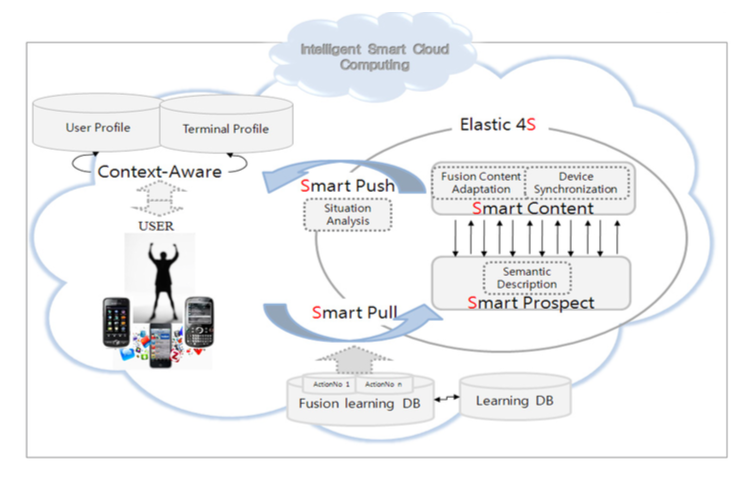
\includegraphics[width=0.5\textwidth]{scc}
    \caption{Smart Cloud Computing Architecture \cite{s110807835}.}
    \label{scc}
  \end{figure}

  Figure \ref{scc} shows how the SCC provides smart learning to the user. It is using Elastic 4S based on information obtained from the user. The information of the user includes the information about the user and the device, received by context-aware sensors. Context-aware monitoring monitors user request(s) and the kind of device(s) that the user is currently using. By using the information collected by the sensors, SCC can provide user-aware service based on Elastic 4S. Elastic 4S is performed through an intelligent learning engine that consists of the rules based on the four services—Smart Pull, Smart Prospect, Smart Content and Smart Push. These four smart services provide high quality services according to the definition of E4S that is described as follows:

  \begin{equation}
    \{E4S_i\}=\{(Spull_i , Spros_i, Scon_i, Spush_i)\}, 1\leq i \leq N
  \end{equation}

  where:

  \begin{itemize}
  \setlength\itemsep{0em}
    \item[] $Spull_i$: Smart pull $—$ analyze the extractable content from the sensing information. 
    \item[] $Spros_i$: Smart prospect $—$ description of the content for target devices and delivery time.
    \item[] $Scon_i$: Smart content $—$ connection establishment between server and target devices.
    \item[] $Spush_i$: Smart push $—$ synchronized delivery of contents to target devices.
  \end{itemize}

  As shown in the definition, the E4S pulls the sensing data and analyzes the extractable contents. The context-aware module is functioning as an information filter that extracts only the intended information from the sensing data. There can be multiple contexts in sensing data depending on the services available in the learning management system. They are individually synchronized and pushed by the smart learning service. The sensing data analysis process identifies the different backgrounds of each learner and accommodates each learner's needs individually. Learning contents are customized based on the background and learning needs. It means that different learning content may have unique technical and functional characteristics and may use different communication channels. Each customized learning contents may differ in modality (i.e., text-based, audio, video, etc.), capability (i.e., bandwidth), and timing (i.e., types of synchronization).

  The system also offers context-aware services, since Context-aware is important \cite{Pratama2014}. A research also contributed to implement context-aware services in educational system \cite{Scott2010}. However, cloud computing were not used as this study only focuses on context-aware in classroom setup only.

  \subsection{Elastic Model}
  The cloud computing enable cloud servers to provide smart learning service to users through additional intelligent processes on existing cloud system. The most important responsibility of the servers is to perform elastic processes such as Elastic Computing for Infrastructure as a Service (IaaS), Elastic Management for Platform as a Service (PaaS) and Elastic Deployment for Software as a Service SaaS) constantly. The elastic processing can be described as collecting user information that is pulled by the sensors in the users' mobile devices and process the pulled information in real-time so that it can accommodate users' changing situation dynamically.

  A study conducted by Kim et al. \cite{Kim2013} proposed the Elastic Conductor that performs provisioning and scheduling for the decision of smart activities. The provisioning and scheduling are performed through an inference engine that utilizes the rules based on three attributes—an object id for user context, a predicate relationship for user behavior, and a value for thinking. The elastic conductor is utilized in PaaS as a smart activity.
  
  The Elastic Conductor it can also generate user interface configurations, such as personalized views and content rendering for each individual user. These processing tasks include four smarts concept: Behavior sensing, Behavior matching, Synchronization and Push – for displays multi-contents on the multi-device or all content on the one device to render learning content. Using sensing context-awareness through the location and IP address of each device, it can orchestrate all devices. Therefore, the multi learning contents can be played in different devices separately to form a \"virtual class\". The architecture of the model is show in the Figure \ref{elastic-conductor}.

  \begin{figure}[htb]
    \centering
    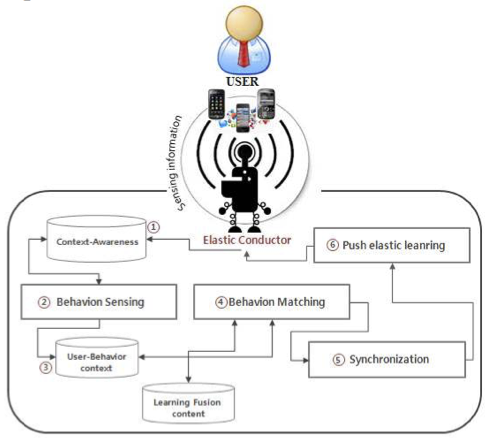
\includegraphics[width=0.3\textwidth]{elastic-conductor}
    \caption{Elastic conductor architecture \cite{Kim2013}.}
    \label{elastic-conductor}
  \end{figure}

  The Figure \ref{elastic-conductor} shows how the conductor provides smart learning to the user. The information of the user included the information about the user and the device, received by context-awareness sensor. Context-awareness monitoring monitors user request(s) and the kind of device(s) that the user is currently using. By using the information collected by the sensors, conductor (1) pulls the sensing information and analyses the extractable contents. The behavior sensing (2) concept is functioning as an information filter that extracts only the intended information from sensing data and (3) storage in the user-behavior context DB. There can be multiple contexts in sensing data depends on the services available in the learning management system. The behavior

  To provide the smart learning service to each individual user, the behavior sensing concept must automatically deduce the actual situation from the user's situation. The behavior sensing is the process of extracting user's behavior information through a variety of sensors to filter information from the sensing information. The filtered information is analyzed to determine user's behavior patterns which the collaboration context information to receive a correct set of user preference, GPS and value of terminal MAC-ID (show the Figure \ref{behaviour-sensing}).

  \begin{figure}[htb]
    \centering
    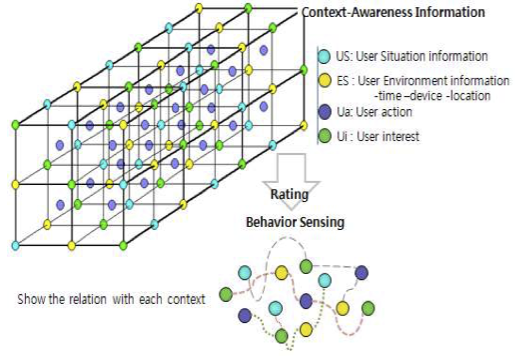
\includegraphics[width=0.4\textwidth]{behaviour-sensing}
    \caption{Behavior sensing domain ontology \cite{Kim2013}.}
    \label{behaviour-sensing}
  \end{figure}

  The filtered process in behavior sensing is defined with the rating function as:

  \begin{equation}
    R: Ua \times Ui \times T \times L \times D \rightarrow Rating
  \end{equation}

  where Ua is user action, Ui is user interest, L is location, T is time, D is device are the information of user situation  and user environment sensing respectively, Rating is the  information of rating. The Ua dimension is defined as Userc U action c U requestc Learning object title and consist of set of user situation. Similarly, the Ui dimensions are defined as Userc U interests U needs c U expertise I experience. The L is defined as Location c Homes Street c Company. The T is defined as Time c Month c Day c Morning c Lunch c- Afternoon c Evening. Finally, the D dimension can be defined as Device c Terminal MAC ID c Application type.

  For instance, continuing $Ua \times Ui \times T \times L \times D$ example considered above, we can define a rating function R on the filtered process $Ua \times Ui \times T \times L \times D$ specifying what a user's request $Ua$ E User action and how much user interested item $Ui$ E User interest at the time T E Time in user's location L e Location and used application type of device D e Device, R(Ua, Ui, T,L,D). Visually, ratings R on the filtered process is can be stored in a multidimensional cube, such as the one shown in Figure \ref{rating}.

  \begin{figure}[htb]
    \centering
    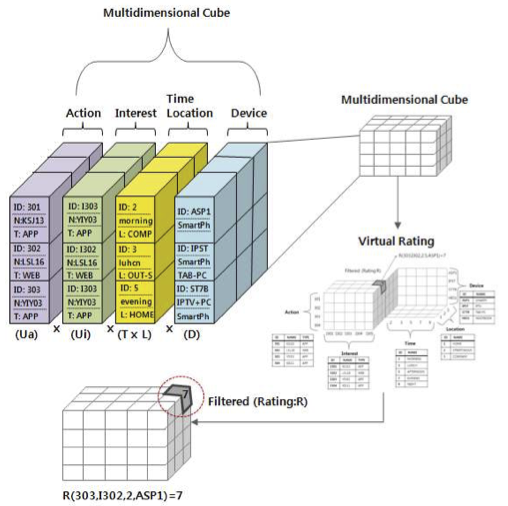
\includegraphics[width=0.4\textwidth]{rating}
    \caption{Rating for the $Ua \times Ui \times T \times L \times D$ in filtered process\cite{Kim2013}.}
    \label{rating}
  \end{figure}

  The double cube in Figure \ref{rating} is stored rating R(Ua, Ui, T, L, D) for the filtered proves $Ua \times Ui \times T \times L \times D$, where the five tables define the sets of user action, interest, location, time and device associated with Action, Interest, Time x Location and Device dimensions respectively.

  For example, the rating R(303,1302,2,ASP1)=7 in Fig. 3 is means that for the action with action ID 303, the user's interest learning object is interest ID 1302 and using this item mainly Time ID 5 in the Location Company, rating was specified during in the device ID ASP1. In other words, the user every afternoon is using application (ID 1302) at the street using smart phone. So that filtered data is basis for creating user behavior database (DB) for providing smart learning service. According to following classification the situation is determine then user behavior database will be created.

  
  \subsection{Cloud and Web 3.0}
  Nasr et al. \cite{nasr2012proposed} proposed an approach of e-learning system that is supported by Paas, Iaas, and Web 3.0. This work is basically using platform provided by Microsoft Windows Azure\footnote{http://azure.microsoft.com/}. As described in this paper, Windows Azure has several important part such as computing part, storage part, fabric controller, Content Delivery Network (CDN), and connect. The parts are depicted in Figure \ref{win-azure}.

  \begin{figure}[htb]
    \centering
    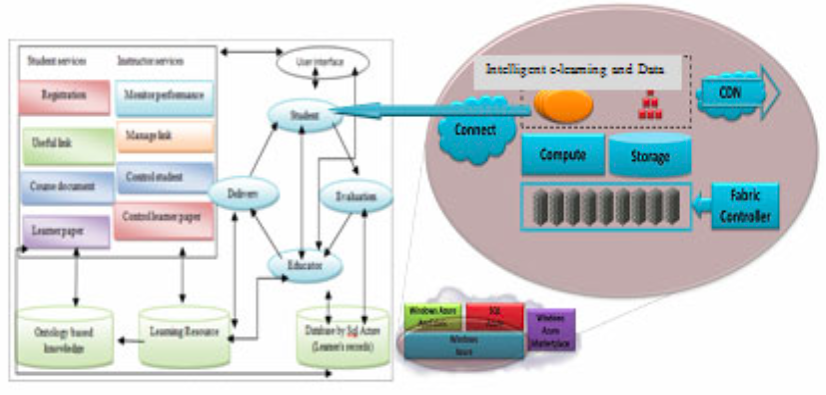
\includegraphics[width=0.4\textwidth]{win-azure}
    \caption{Windows Azure provides compute and storage services for intelligent e-learning in the cloud \cite{nasr2012proposed}.}
    \label{win-azure}
  \end{figure}

  The development of e-learning cannot ignore the cloud computing and Web3.0 trends. There are many benefits from using the integration between cloud computing and Web3.0 for e-learning. Using cloud computing and Web3.0 for e-learning influences the way an e-learning software projects are managed. There are specific tasks that deal with finding providers for cloud computing, depending on the requirements (infrastructure, platform or services). Also, the cost and risk management influences the way the e-learning based on integrating the cloud computing and Web3.0 are managed. An intelligent e- learning system based on an integration between cloud computing and web 3.0 has been developed in order to enhance the efficiency of learning environment, provide flourish; growing, up-to-date, self-regulated, stability, QoS-guaranteed (Quality of Service), equilibrium, reliability, scalability, time reduction, efficient resource use, flexibility, and sustainability of e- learning system. In the future we wish to develop an e-learning by using an integration between web 4.0 and cloud computing.

  \subsection{Content Oriented}
  This paper proposed a content-oriented smart education system based on cloud computing that integrates a number of features required for implementing a cloud-based educational media service environment. The aim was to develop a total, integrated education content service system based on cloud computing to deliver and share a variety of enhanced forms of educational content, such as text, images, video, audio, animations, memos, quizzes, and 3D and AR objects. For the realization of a cloud- based content service system, we developed six main features. First, by leveraging several IT and cloud computing technologies, we established a private cloud platform to install and operate a cloud-based educational media service environment. In addition, we identified the software and applications required for the proposed cloud-based education services. Second, we developed a common file format enabling manipulation of various forms of media content on multiple platforms using XML, WebGL, and HTML5. Third, we implemented an authoring tool, allowing teachers to create various types of smart media content, including text, images, pictures, videos, and 3D and AR objects. Fourth, we developed a content viewer to display media content on diverse types of devices, such as PCs, notebooks, netbooks, tablets, smart TVs, and smartphones, through a multi-platform based design. Fifth, we implemented an inference engine to provide students with customized individual learning content by analyzing their learning and content usage patterns. Sixth, a security system was included in the proposed system to encrypt data and to control user access for dependable smart media content services \cite{jeong2013content} \cite{jeong2013cloud}.

  Figure \ref{archi} presents the proposed cloud-based education system for smart media content services [12, 14]. The proposed system enables delivery and sharing of a variety of enhanced educational content by integrating a number of features required for the deployment of a cloud-based educational media service environment. Figure 2 shows the proposed system with its six main features required for deploying cloud-based educational content service.

  \begin{figure}[htb]
    \centering
    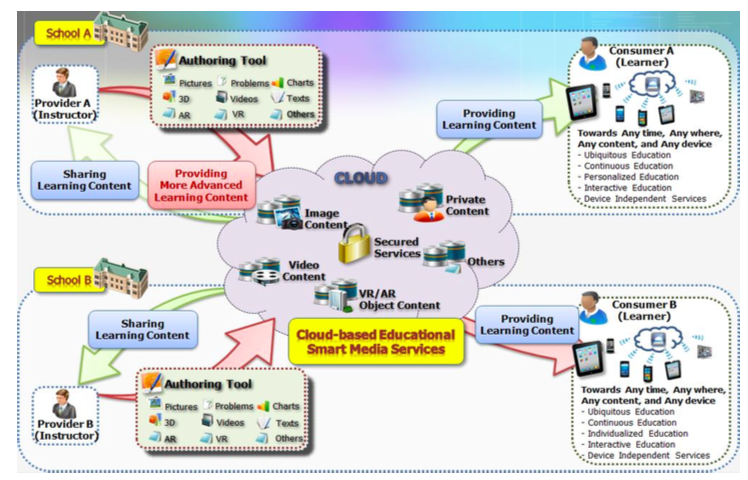
\includegraphics[width=0.5\textwidth]{content-oriented-archi}
    \caption{Architecture of the proposed cloud-based education system for smart content services \cite{jeong2013content}.}
    \label{archi}
  \end{figure}
  
  Teachers in schools are able to create various forms of learning content, including text, images, video, 3-dimensional (3D) objects, and virtual scenes based on virtual reality (VR) and augmented reality (AR), using an authoring tool provided by the system. The content is managed in the cloud in a compatible common file format. The system supports various platforms, such as personal computers (PCs), notebooks, tablets, smart TVs, and smart phones. The system also provides a content viewer for displaying learning content and an inference engine to support content customized to each individual student, based on their preferences and knowledge. An inference engine is included to provide students with personalized learning content by analyzing their preferences, learning styles, and content usage patterns. In addition, a security system is provided for controlling data access and encryption in the cloud.

  \begin{figure}[htb]
    \centering
    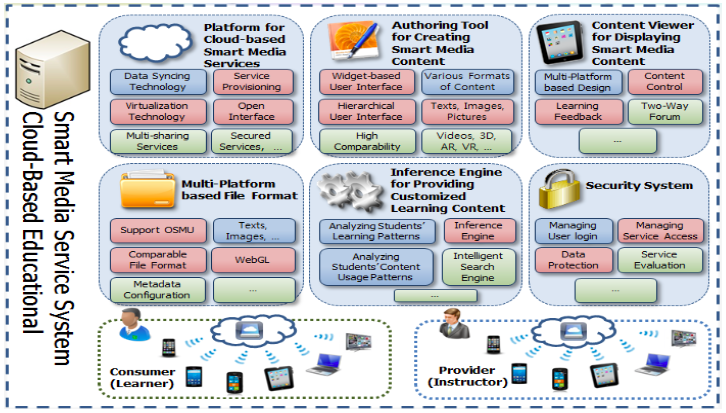
\includegraphics[width=0.5\textwidth]{content-oriented-feature}
    \caption{Infrastructure of the proposed system with its six main features \cite{jeong2013content}.}
    \label{feature}
  \end{figure}

  Cloud Platform: The proposed system established a private cloud platform to provide an infrastructure for the implementation of a cloud-based educational media service environment by applying several IT and cloud computing technologies, such as data synchronization, virtualization, service provisioning, and multi-sharing services. In other words, we configured a private cloud platform to install and operate a cloud-based educational media service environment by leveraging IT and cloud computing technologies. In addition, we identified software and applications required for the proposed cloud-based education service and allocated them to the three cloud service models (IaaS, PaaS, and SaaS) as shown in Figure 3.

  We developed a common file format to be able to manipulate various types of media content on multiple device platforms based on an XML document format with HTML5, eXtensible 3-Dimensional (X3D), and JavaScript.
  
  XML has been used in many areas as a means of representing data and meta-data. It consists of two components: the Document Type Definition (DTD) that defines the schema for the XML document structure and the eXtensible Style sheet Language (XSL) that describes styles for representing XML data. That is, XML separately represents content and style, so that the same content can be viewed on multiple devices by defining only the styles appropriate to each device. XML is also designed to make it easy not only to describe many different kinds of data but also to send and receive data between computer systems connected to the Internet, such as data transmission in smartphones [13]. For these reasons, we adopted XML as the basic representation language for developing a common file format for various types of contents. Table 1 summarizes the content types defined in the common file format [13]. These content types are inserted and handled in a document file as a control. We divided the content types into two categories: basic controls that are displayed in a 2D screen and interactive controls that can play 3D video and objects or respond to user actions. Each of these controls is defined with a number of properties and each property is specified with its own data type, such as numeric, character, or multiple choice. Table 2 shows the properties and provides brief explanations of each control defined in the common file format.

  Authoring Tool: The system provides an authoring tool to allow teachers to create various types of smart media content including text, images, video, sounds, widgets, and 3D, VR, and AR objects and scenes. Figure 4 shows the content creation processes of the authoring tool system. The content creation process is divided into three phases: control creation, file configuration and editing, and distribution. In Phase 1, users can perform operations to create controls (content) to be inserted in documents. In Phase 2, users can set the layout of a document and then insert controls into the document. In Phase 3, the authoring system converts the newly-created document to the common file format then uploads the file to the server for distribution to client devices. The document structure of the authoring tool system follows the structure of the Flow Document of WPF (Windows Presentation Foundation). Figure 5 shows examples of a document creation process (Phase 2) using text and image controls (contents).

  Content Viewer: We developed a content viewer to display media on multiple platforms. Figure 6 shows a number of devices supported by the content viewer. The contents created by the authoring tool are saved in the XML-based common file format described in Section 3.2.2. The viewer displays content on each device by converting the XML data to HTML, appropriate to each device. We used XSLT (Extensible Style sheet Language Transformations) for the file format conversion. XSLT is a language for transforming XML documents into other file formats. The content of the basic controls specified in Table 1 can be easily converted to HTML format via XSLT. However, it is difficult to covert the XML data of the interactive control content (i.e., audio, animations, 3D objects) to HTML format with XSLT. To solve this problem, we create an HTML area for displaying an interactive control, and then display the corresponding content on the HTML area through another content viewer we developed for visualizing interactive controls [13]. Figure 7 shows an example of learning content displayed on an iOS-based smartphone [13].

% disguise this part, bcs this is really important part, dont mess with it
\section{Discussion}
% describe: what drives a successful e-learning comprehensively
% and reflects to the papers.
Some benefits of cloud computing in education are drawn in a study by Gonzalez et al. \cite{Gonzalez-Martinez2014}. Those advantages are a wealth of online application to support education, flexible creation of learning environments, support for mobile learning, computing-intensive support for teaching, learning, and evaluation, scalability of learning systems and applications, costs saving in hardware, cost saving in software.

This study tries to evaluate the above mentioned approach of cloud computing in smart learning system based on a study presented by Sun et al. \cite{Sun2008}. That work alleged that there are some factors that push a e-learning system to be successful. The work collected nearly 300 questionnaire and a stepwise multiple regression analysis was conducted to extract some potential information. The result showed that the factors are learner's computer anxiety, instructor attitude toward e-Learning, e-Learning course flexibility, e-Learning course quality, perceived usefulness, perceived ease of use, and diversity in assessment are the critical factors affecting learner's perceived satisfaction \cite{Sun2008}. However, since our study only tries to investigate the technical implementation of cloud computing without the involvement of students, instructors, or courses, factors that are possible to be used are only flexibility and assessment. Furthermore, in order to evaluate the approaches deeper, we add some more factors that are relevant with smart learning system, such as context-awareness, security, multi-media support, and ontology utilization.

% smart cloud computing
Kim et al. presented a smart learning services that is based on Smart Cloud Computing (SCC). As mentioned above, this approach offers smart learning services through 4S model, which are smart push, smart . Security feature is also covered in this approach, although it is just securing user's personal information through some security setting without data encryption. SCC also manages to implement context-awareness by utilizing context-aware sensors. The context-aware module considers the characteristics of each user individually, such as learners' knowledge interests, needs, expertise, and experiences. Thus it can provide highly customized and relevant learning services to each user. Each cloud type (Iaas, Paas, Saas) are covered using smart cloud approach. Furthermore, no specific platform are used in this approach, this will lead in to a good flexibility. Semantic description based on UVA (Universal Video Adaptation) are used to provide accurate and meaningful information for the fusion content (content-database). The paper also managed to show the implementation with four fusion media, which includes video, audio, PPT, and text.

% elastic model
Elastic Model (EM) \cite{Kim2013} focuses to intelligently meet users' need. The approach is slightly similar with the SCC because EM also use the four smart concept to cloud service. This proposed system also support multiple devices just as SCC approach. Furthermore, this system is independent from any platform and this make this approach has a good flexibility. Security factor is also slightly described to secure each user's personal information using some security setting e.g. user's schedule and location. This approach also utilizes context-aware by implementing behavior sensing to provide smart learning service to each individual user. However, there are no ontological approach explained in the paper. 

% ontology
The approach from Nasr et al. \cite{nasr2012proposed} integrates cloud computing as a platform with the help of Web 3.0 to build intelligent learning system. This is done by making use Windows Azure as the platform for the system. The system also proposed ontology based model. For implementing the knowledge the leaning resources have to be described by means of meta-data. This is also a resource for contextual learning. Security system in this approach is fully covered in Windows Azure platform that obviously has the enterprise level security system. However, this approach does not mention any description in multi device support and since this system depends on Windows Azure platform to be developed this system is more likely to be having less flexibility.

% content-oriented
Content-oriented approach \cite{jeong2013content} to make use of cloud computing in smart education system integrates a number of features that will enable a school to deliver and share a variety of enhanced forms of educational content including text, images, videos, and even 3D or even virtual scenes. Thus, this approach has a rich amount of contents and does support multimedia content. Moreover, this content-oriented approach also support multiple-device with multiple screen size and features. This concept also offers a security system, the author mentioned that to encrypt data and control privileged user access but also to protect and solve network problems in the cloud. An inference engine is utilized to provide students with personalized learning content by analyzing their preferences, learning styles, and content usage patterns. This proposed system does not use ontological approach to model the educational database or user preference. However, this system offers flexibility as it utilizes XML for data and document exchange and it also develops Common File Format to be able to manipulate various types of media content on multiple device platforms. Although this approach seems to have a comprehensive concept of cloud computing in smart learning system, this proposed concept has not been fully implemented yet.

% Factors in implementation of cloud computing \cite{morgan2013factors}

To sum up the above discussion, Table \ref{tab:comparison} depicts the four approach in summary:

\begin{table}[htb]
  \caption{This table shows some data}
  \label{tab:comparison}
  \scriptsize
  \begin{center}
  \begin{tabular}{lcccc}
     & SCC & EM & Web 3.0 & Content-oriented \\
    \hline
    Security & \cmark & \cmark & \cmark & \cmark \\
    Context-awareness & \cmark & \cmark & \cmark & \cmark \\
    Multi-device support & \cmark & \cmark & $-$ & \cmark \\
    Ontology & \cmark & $-$ & \cmark &  $-$ \\
    Flexibility & \cmark & \cmark &  $-$ & \cmark
  \end{tabular}
  \end{center}
\end{table}

  % draw a table about whole comparison, as f alsaif did on her paper
From Table \ref{tab:comparison}, we can conclude that SCC has all factors that the author wants to assess. Some other approaches lack in one or two factor and there are no approach that lacks three or more factors.

Moreover, in order to deliver an effective and successful smart learning system, intuitive user interface and an out of the box user experience that will make the system easier to be used might be factors that has to be keep in mind since it is mentioned in \cite{Sun2008} that ease of use is one factor that drives a successful learning system. To sum up, the author suggests that adaptation of cloud computing in smart learning system can be said successful if it is abele to prevent duplication of data and can manage computing resources efficiently.

\section{Concluding Remarks}
Cloud computing services offer several advantages in its implementation to e-learning system, such as increased cost savings and also improved efficiency and convenience of educational services. Furthermore, e-learning services can be also enhanced to be smarter and more efficient using context-aware technologies as context-aware services are based on the users behavior. This paper has compared and reviewed several researches and articles about cloud computing services in smart learning environment in terms of context-awareness, security, ontology, multi-device support, and flexibility. These factors are drawn out from a research that tried to determine factors that drive the successfulness of e-learning\cite{Sun2008}. The result showed that there is only SCC approach that is able to cover all factors used in assessment.

Further studies with regard to cloud computing should in smart learning system should consider security as an important issue as users' information are stored in the system. Encryption can be taken into account for improving the security of the system and to protect personal data from any unwanted access. The comprehensive survey are needed to be undertaken in order to assess the capability and the usefulness of the system. Moreover, a benchmark about how system runs will show the benefits and how efficient cloud computing has made the smart learning system become. To sum up, further studies, which take more variables into account, will need to be undertaken.

% \acknowledgements{
% The authors wish to thank Dr. for the help on this work.}

\bibliographystyle{unsrt}
%%use following if all content of bibtex file should be shown
% \nocite{*}
\bibliography{sc2015}
\end{document}
